\chapter{Analýza robustnosti a štrukturálnej zraniteľnosti siete letísk}
\label{robustness_analysis}

V tejto kapitole analyzujeme robustnosť a štrukturálnu zraniteľnosť siete letísk. Najprv sa bližšie pozrieme na základné súvisiace štatistiky siete, ako sú napr. hustota siete, asortativita alebo počet artikulácii a mostov. Následne sa zameriame na analýzu toho, ako tieto štrukturálne charakteristiky ovplyvňujú sieť a jej robustnosť pri náhodných a cielených útokoch.

\section{Základné štrukturálne charakteristiky siete letísk}

Skôr než sa pozrieme na samotnú analýzu robustnosti, je potrebné porozumieť základným štrukturálnym vlastnostiam skúmanej siete. Ako už bolo spomenuté v predchádzajúcich kapitolách, tento orientovaný graf obsahuje $3214$ vrcholov a $36907$ hrán.

Ak sa zameriame na \textbf{hustotu siete}, ktorá je definovaná ako podiel skutočného počtu hrán voči maximálnemu možnému počtu hrán, zisíme, že, ako aj pre iné dopravné siete, aj pre sieť letísk platí, že je veľmi riedka. Konkrétne, hustota siete je iba $0.36\%$.

Ďalšou dôležitou charakteristikou je \textbf{asortativita}, ktorá vyjadruje, či sa vrcholy s podobným stupňom prepájajú častejšie medzi sebou. V našom prípade dosahuje hodnota asortativity približne $-0.019$, teda je veľmi blízka nule. To naznačuje, že sieť nevykazuje výraznú tendenciu spájať letiská s podobným alebo odlišným počtom spojení.

Napokon sme analyzovali aj \textbf{reciprocitu siete}, ktorá vyjadruje podiel obojstranných spojení. Hodnota reciprocity v sieti letísk je $97.81\,\%$, čo znamená, že letecká sieť je takmer symetrická.

\section{Listy, artikulácie a mosty}
Vďaka takmer úplnej symetrii siete, pri tejto analýze uvažujeme neorientovanú verziu grafu. Tá obsahuje $718$ \textbf{listov} (pozri \ref{fig:leaves}). Zaujímavé však je, že ak by sme sa pozreli na orientovaný graf, takýchto letísk by bolo len $31$ (berúc do úvahy letíská kam sa iba prilieta, alebo z ktorých sa iba odlieta). V týchto letiskách sme však nenašli žiaden vzorec, orem toho, že väčšina z nich sa nachádza v štáte \textbf{Alijaška}.

\begin{figure}[H]
    \centering
    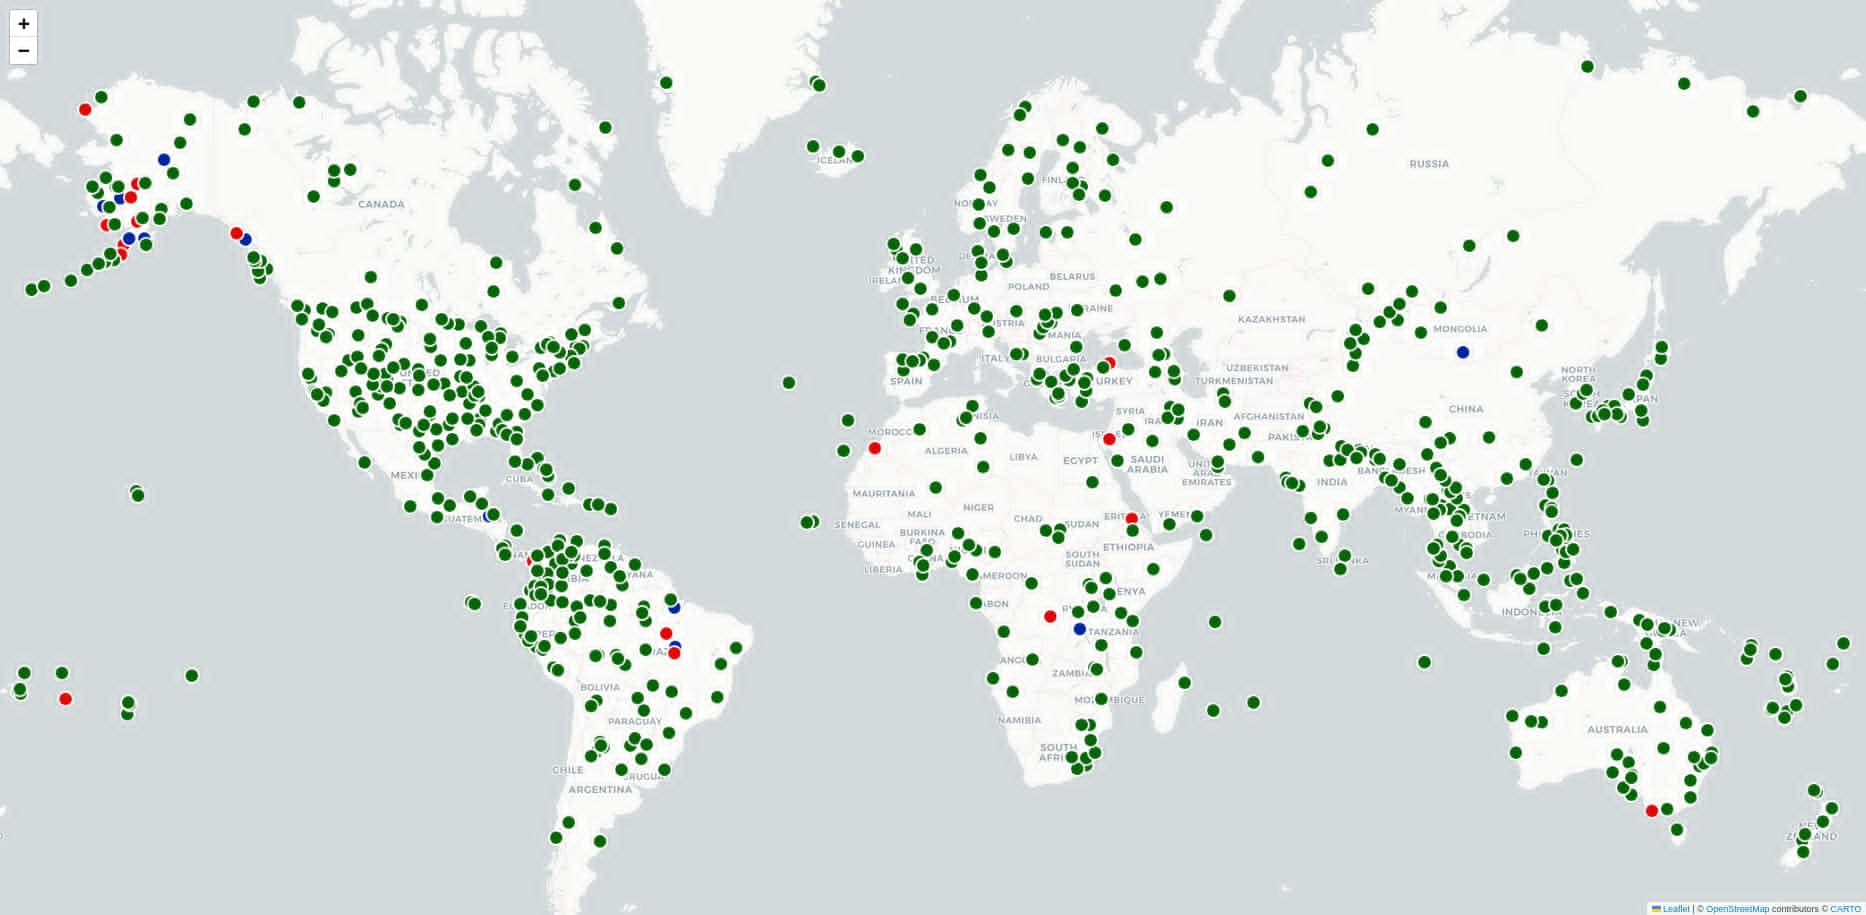
\includegraphics[width=0.9\linewidth]{images/fig_leaves.jpg}
    \caption{\centering Vizualizácia listov siete letísk (zelenou farbou). Modrou farbou sú zobrazené letiská, kam sa dá iba priletieť, naopak, červenou letiská, odkiaľ sa iba odlieta.}
    \label{fig:leaves}
\end{figure}

Ďalšou zaujímavou charakteristikou sú artikulácie, teda vrcholy, po ktorých odstránení sa zvýši počet komponentov v stieti. V sieti letísk sa takýchto vrcholov nachádza $333$. Mostov, ktoré nám naopak hovoria o hranách po ktorých odstránení sa počet komponentov zvýši, je oveľa viac, a to $757$. To naznačuje, že jedna artikulácia môže byť v tomto prípade spojená s viac ako jedným mostom (v pieremere $2.27$). Všetky mosty v tejto sieti sú znázornené na Obrázku~\ref{fig:bridges}.

V sieti letísk sa ukázalo, že až $716$ z mostov je spojených práve s listom, čo znamená že ..

Ak sa pozrieme na artikulácie, najviac ich je v štátoch \textbf{USA} a \textbf{Brazílii} a \textbf{Kanade}. Tieto tri krajiny sa však nachádzajú aj v top 4 krajinách s najväčším počtom letísk. Z toho dôvodu sme sa rozhodi pozrieť sa na to, či sa počet artikulácií v jednotlivých krajinách súvisí v počtom letísk. Korelačný koficient je $0.97$, čo naznačuje, že tieto dve veci sú veľmi silno korelované.

Zaujímavé môže byť, že artikulácie zvyknú máť oveľa vyšší stupeň vrchola než je priemer (pozri Podkapitolu~\ref{kubko}), a to $39.6$ aj ako vrcholy, ktoré nie sú artikuláciami, ktorých priemerný stupeň je $8.5$.

\begin{table}[H]
    \centering
    \begin{tabular}{l c}
        \toprule
        \textbf{Letisko}                   & \textbf{Impact} \\
        \midrule
        El Dorado International Airport    & 18              \\
        Denver International Airport       & 15              \\
        Tokyo Haneda International Airport & 14              \\
        Jorge Newbery Airpark              & 13              \\
        Ninoy Aquino International Airport & 13              \\
        \bottomrule
    \end{tabular}
    \caption{Top 5 letísk, po ktorých odstránení pribudne v sieti najviac nových komponentov.}
    \label{tab:top_impact_airports}
\end{table}


Pozrime sa však ešte bližšie na artikulácia a konkrétne, na impact, ktorý ich odstraňovanie bude mať. Tabuľka~\ref{tab:top_impact_airports} nám ukazuje, top 5 artikulácii, po ktorých odstránení sa počet komponentov najviac zvýši. Na prvom mieste sa nachádza letisko \textbf{El Dorado International Airport} v Kolumbii, po ktorého odstránení zo siete by nám pribudlo $18$ nových komponentov.

\section{Analýza robustnosti siete letísk}

\subsection{Odstraňovanie vrcholov}

Na Obrázkoch 3.2 a 3.3 môžeme pozorovať správanie siete pri postupnom odstraňovaní vrcholov rôznymi stratégiami (náhodné odstraňovanie, cielené odstraňovanie závisiace od vrchola s najvyšším stupňom, artikulácie a betweenness centrality, aj v dynamických variantoch, kde sa tieto štatistiky znova prepočítajú po každom odstránení vrchola zo siete). Ako metriku robustnosti sme použili relatívnu veľkosť najväčšieho súvislého komponentu, zatiaľ čo fragmentáciu siete charakterizuje počet komponentov siete.

Najodolnejšia sa ukazuje sieť pri náhodnom odstraňovaní vrcholov, kde veľkosť najväčšieho komponentu klesá pomerne pomaly. Naopak, cielené odstraňovanie kritických vrcholov vedie k výrazne rýchlejšej fragmentácii siete, pričom nedynamické verzie (kde sa odstraňujú vrcholy iba na základe počiatočnej siete), už výrazne rýchlejšie vedú k zmenšovaniu najväčšieho komponentu. Najväčší dopad však majú dynamické stratégie založené na artikuláciách, betweenness centralite a stupni vrchola, pri ktorých dochádza k prudkému poklesu veľkosti najväčšieho komponentu a prudkému nárastu počtu komponentov už po odstránení relatívne malej časti letísk.

\begin{figure}[htpb]
    \centering
    % Prvý obrázok
    \begin{minipage}[b]{0.48\textwidth}
        \centering
        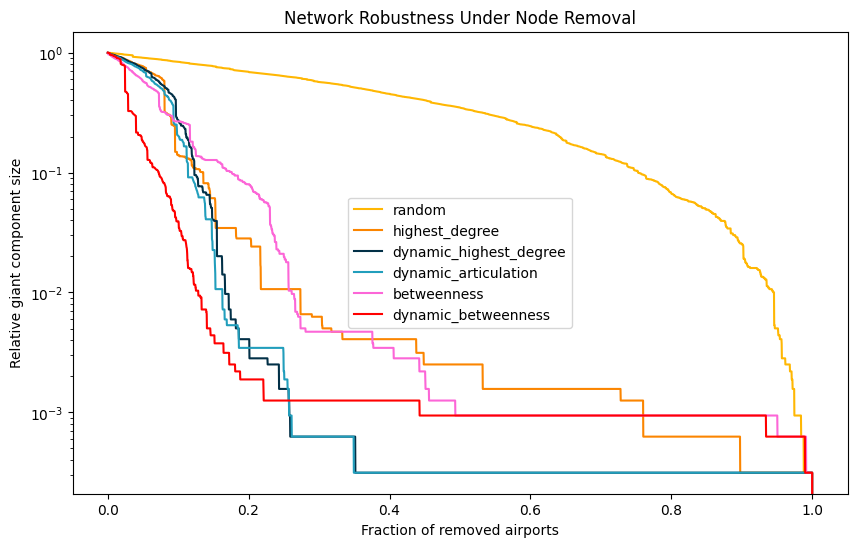
\includegraphics[width=\textwidth]{images/network_robustness_under_node_removal_log.png}
        \caption{Porovnanie robustnosti siete pri rôznych stratégiách odstraňovania vrcholov pomocou relatívnej veľkosti najväčšieho súvislého komponentu.}
        \label{fig:xz_wl_dist}
    \end{minipage}
    \hfill
    % Druhý obrázok
    \begin{minipage}[b]{0.48\textwidth}
        \centering
        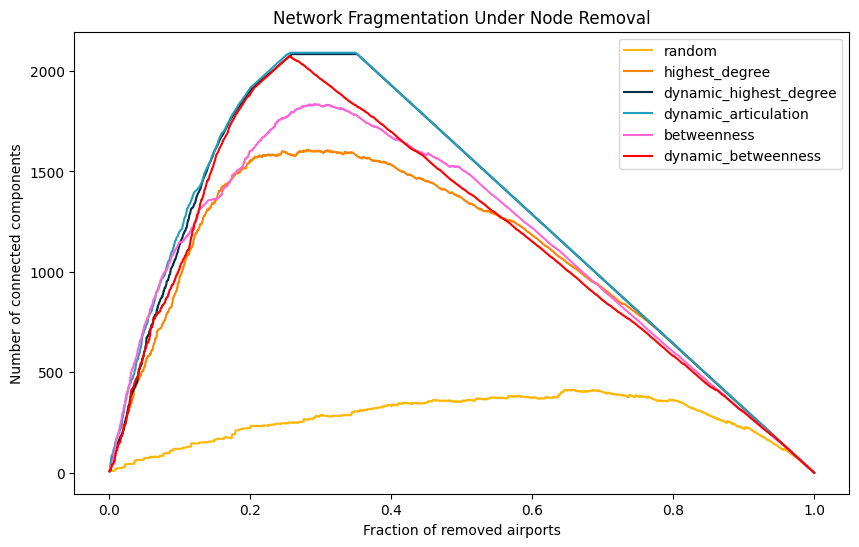
\includegraphics[width=\textwidth]{images/network_fragmentation_under_node_removal.png}
        \caption{Porovnanie fragmentácie siete pri rôznych stratégiách odstraňovania vrcholov pomocou počtu súvislých komponentov.}
        \label{fig:xz_whole_dist}
    \end{minipage}
\end{figure}

Ako najefektívnejšia sa ukazuje stratégia odstraňovania vrcholov pomocou dynamicky, na základe ich betweenness centrality. Dynamické odstraňovanie pomocou najvyšieho stupňa a artikulácie sa správajú veľmi podobne a je tažké rozoznať ktorá z nich je efektívnejšie.

Preto sme zhotovili Tabuľku~X, ktorá ukazuje, vypočítanú plochu pod krivkou (AUC) pre každú z týchto stratégií, ktorá nám umožňuje lepšie porovnať ich efektivitu.



%BUDE TABUľKA

%BRIDGES
\subsection{Odstraňovanie hrán}

Pri odststraňovaní mostov sa ukázalo, že odstraňovanie mostov vedie k výrazne pomalšej redukcii veľkosti najväčšieho komponentu, než odstaňovanie vrcholov.

V tejto časti porovnávame dve stratégie. Prvou je náhodné odstraňovanie hrán. Druhou je dynamická verzia odstaňovania mostov, teda v každom kroku sa nájdu aktuálne hraný ktoré sú msostami.

Výsledok, znázornený na Obrázku~X ukazuje, že odstraňovanie mostov, samozrejme, vedie rýchlejšiemu rozpadu siete. Pri tejto stratégii môže byť zaujímavé pozorovať správanie krivky v grafe, kde veľkosť najväčšieho komponentu spočiatku klesá lineárne, ale následne sa zaství a je dlhý čas konštantná. Je to tak preto že na začiatku sa postupne odstraňovali všetky mosty až do chvíle, kedy už neostali žiadne. Tam algoritmus prešiem na stratégiu odstraňovania náhodných hrán a kedže žiadne mosty neexistovali, najväčší komponent sa nemal ako zmenšovať, a ani sieť sa nemala ako fragmentovať na menšie časti. V bode, kedy už bolo odstránených viac ako polovica hrán zo siete sa táto situácia zasa zvrhla na odstraňovanie mostov, ktoré viedlo k rapídnemu pokledu veľkosti najväčšieho komponentu a zvyšovaniu fragmentácie siete.
